% !TeX spellcheck = en_US
%\documentclass[11pt,a4paper]{article}
\documentclass[11pt
  , a4paper
  , article
  , oneside
%  , twoside
%  , draft
]{memoir}

\usepackage{control}
\usepackage{kotex}
\usepackage[numbers]{natbib}
%\usepackage[pdftex]{graphicx}
%\DeclareGraphicsExtensions{.pdf,.png,.jpg}
\begin{document}

\newcommand{\technumber}{
  Digital Signal Processing using MATLAB\\
  Document 1: 2016-03-26}
\title{\textbf{Digital Signal Processing: 실습 6 \\
		제3장 이산시간 푸리에  변환의 성질 \\}}

\author{이상일\thanks{silee7103@ibs.re.kr} \\

  학번: 201460437\\
  Computer Engineering, Chungnam National University 
}
\date{\today}

\renewcommand{\maketitlehooka}{\begin{flushright}\textsf{\technumber}\end{flushright}}
%\renewcommand{\maketitlehookb}{\centering\textsf{\subtitle}}
%\renewcommand{\maketitlehookc}{C}
%\renewcommand{\maketitlehookd}{D}

\maketitle

\begin{abstract}
MATLAB을 사용한 Digital Signal Processing에 대한 실습과제에 대한 Documents를 구성한다.
\end{abstract}

\chapter{Example 3-18:}

\begin{lstlisting}[style=termstyle]
% Example 3.18
dt = 0.00005; t = -0.005:dt:0.005; xa = exp(-1000*abs(t));
Wmax = 2*pi*2000; K = 500; k = 0:1:K;
W = k*Wmax/K;
Xa = xa * exp(-j*t'*W) * dt; Xa = real(Xa);
W = [-fliplr(W), W(2:501)];
Xa = [fliplr(Xa), Xa(2:501)];
subplot(2,1,1);plot(t*1000,xa);
xlabel('t in msec.'); ylabel('xa(t)')
title('Analog Signal')

subplot(2,1,2);plot(W/(2*pi*1000),Xa*1000);
xlabel('Frequency in KHz'); ylabel('Xa(jW)*1000')
title('Continuous-time Fourier Transform')
\end{lstlisting}

\begin{figure}[h!]
	\centering
	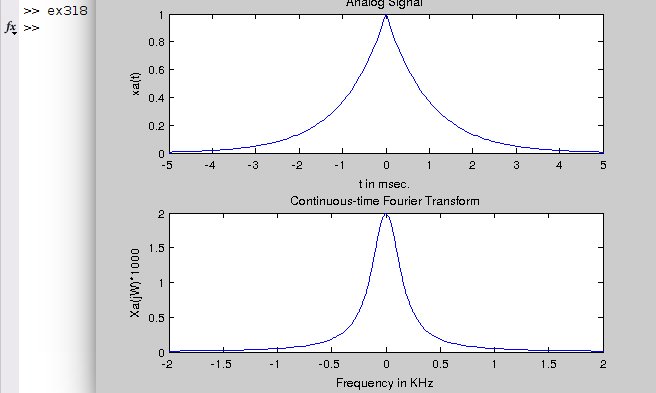
\includegraphics[width=0.7\textwidth,height=0.4\textwidth]{./images/ex318.png}
	\caption{Example 3.18 Result}
	\label{fig:Example 3-18 Result}
\end{figure}

\chapter{Example 3-19a:}

\begin{lstlisting}[style=termstyle]
% Example 3.19a
dt = 0.00005; t = -0.005:dt:0.005; 
xa = exp(-1000*abs(t));

Ts = 0.0002; n = -25:1:25; x = exp(-1000*abs(n*Ts));
K = 500; k = 0:1:K;
w = pi*k/K;

X = x * exp(-j*n'*w);
X = real(X);
w = [-fliplr(w), w(2:K+1)];
X = [fliplr(X), X(2:K+1)];

subplot(2,1,1);plot(t*1000,xa);
xlabel('t in msec.'); ylabel('x1(n)')
title('Discrete Signal'); hold on

stem(n*Ts*1000,x); gtext('Ts=0.2 msec'); hold off

subplot(2,1,2);plot(w/pi,X);
xlabel('Frequency in pi units'); ylabel('X1(w)')
title('Discrete-time Fourier Transform')
\end{lstlisting}

\clearpage

\begin{figure}[h!]
	\centering
	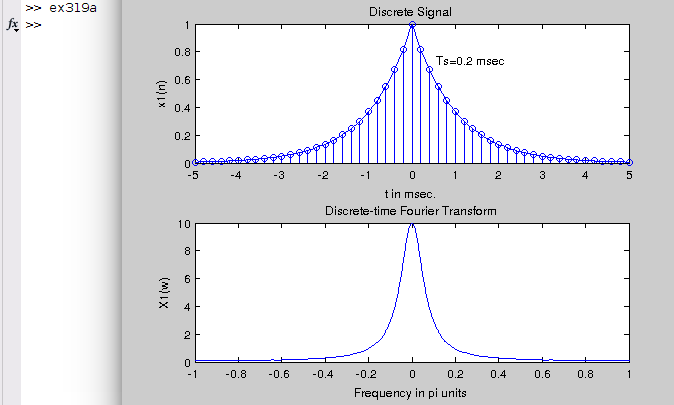
\includegraphics[width=0.7\textwidth,height=0.5\textwidth]{./images/ex319a.png}
	\caption{Example 3.19a Result}
	\label{fig:Example 3-19a Result}
\end{figure}

\clearpage

\chapter{Example 3-19b:}
\begin{lstlisting}[style=termstyle]
% Example 3.19b
dt = 0.00005; t = -0.005:dt:0.005; xa = exp(-1000*abs(t));
Ts = 0.001; n = -5:1:5;
x = exp(-1000*abs(n*Ts));
K = 500; k = 0:1:K;
w = pi*k/K;
X = x * exp(-j*n'*w);
X = real(X);
w = [-fliplr(w), w(2:K+1)];
X = [fliplr(X), X(2:K+1)];

subplot(2,1,1);plot(t*1000,xa);
xlabel('t in msec.'); ylabel('x2(n)')
title('Discrete Signal'); hold on

stem(n*Ts*1000,x); gtext('Ts=1 msec'); hold off

subplot(2,1,2);plot(w/pi,X);
xlabel('Frequency in pi units'); ylabel('X2(w)')
title('Discrete-time Fourier Transform')
\end{lstlisting}

\begin{figure}[h!]
	\centering
	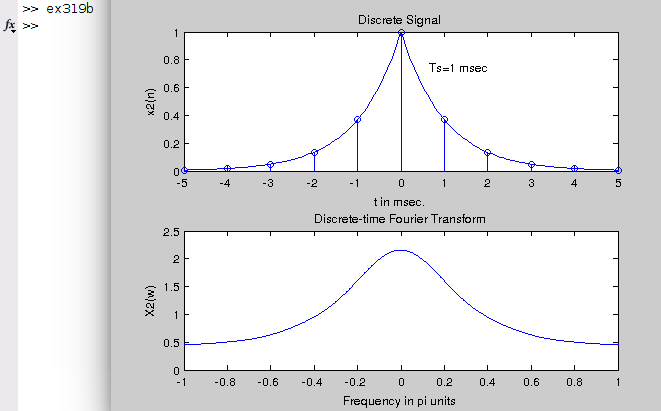
\includegraphics[width=0.7\textwidth,height=0.35\textwidth]{./images/ex319b.png}
	\caption{Example 3.19b Result}
	\label{fig:Example 3-19b Result}
\end{figure}

\chapter{Example 3-21:}
\begin{lstlisting}[style=termstyle]
% Example 3.21
ts = 0.0002; Fs = 1/ts; n = -25:1:25; nTs = n*ts;
x = exp(-1000*abs(nTs));
dt = 0.00005;
t = -0.005:dt:0.005;

xa = x * sinc(Fs*(ones(length(nTs),1)*t-nTs'*ones(1,length(t))));
error = max(abs(xa - exp(-1000*abs(t))))

subplot(2,1,2);plot(t*1000,xa);
xlabel('t in msec.'); ylabel('xa(t)')
title('Reconstructed Signal from x1(n) using sinc function'); hold on
stem(n*ts*1000,x); hold off
\end{lstlisting}

\clearpage

\begin{figure}[h!]
	\centering
	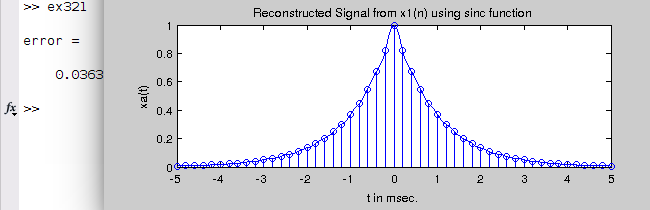
\includegraphics{./images/ex321.png}
	\caption{Example 3.21 Result}
	\label{fig:Example 3-21 Result}
\end{figure}

\chapter{Example 3-22:}
\begin{lstlisting}[style=termstyle]
% Example 3.22
ts = 0.001; Fs = 1/ts; n = -5:1:5; nTs = n*ts;
x = exp(-1000*abs(nTs));
dt = 0.00005;
t = -0.005:dt:0.005;

xa = x * sinc(Fs*(ones(length(nTs),1)*t-nTs'*ones(1,length(t))));
error = max(abs(xa - exp(-1000*abs(t))))

subplot(2,1,2);plot(t*1000,xa);
xlabel('t in msec.'); ylabel('xa(t)')
title('Reconstructed Signal from x2(n) using sinc function'); hold on
stem(n*ts*1000,x); hold off  
\end{lstlisting}

\begin{figure}[h!]
	\centering
	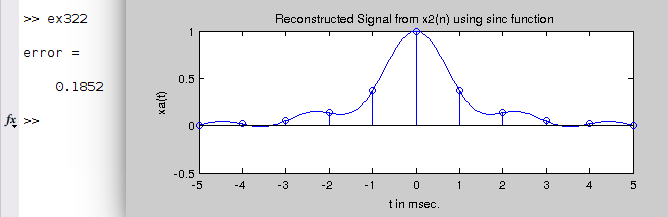
\includegraphics[width=0.7\textwidth,height=0.4\textwidth]{./images/ex322.png}
	\caption{Example 3.22 Result}
	\label{fig:Example 3-22 Result}
\end{figure}

\chapter{Example 3-23:}
\begin{lstlisting}[style=termstyle]
% Example 3.23
ts = 0.0002; n = -25:1:25; nTs = n*ts;
x = exp(-1000*abs(nTs));

subplot(2,1,1); stairs(nTs*1000,x);
xlabel('t in msec.'); ylabel('xa(t)')
title('Reconstructed Signal from x1(n) using zero-order-hold'); hold on
stem(n*ts*1000,x); hold off

subplot(2,1,2); plot(nTs*1000,x);
xlabel('t in msec.'); ylabel('xa(t)')
title('Reconstructed Signal from x1(n) using first-order-hold'); hold on
stem(n*ts*1000,x); hold off
\end{lstlisting}

\begin{figure}[h!]
	\centering
	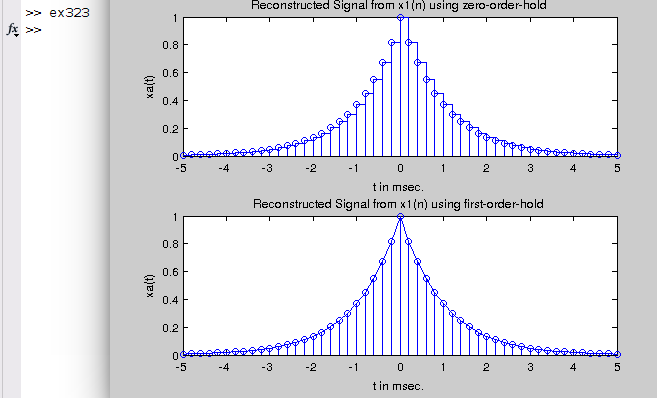
\includegraphics[width=0.7\textwidth,height=0.4\textwidth]{./images/ex323.png}
	\caption{Example 3.22 Result}
	\label{fig:Example 3-23 Result}
\end{figure}

\clearpage

\chapter{Problem 3-17:}
\begin{lstlisting}[style=termstyle]
%Problem 3.17

\end{lstlisting}


\chapter{Problem 3-18:}
\begin{lstlisting}[style=termstyle]
%Problem 3.18

\end{lstlisting}

\end{document}

